% -*-coding: utf-8 -*-
\documentclass[compress,mathserif]{beamer}

\usepackage[utf8]{inputenc}
\usepackage[english]{babel}
\usepackage[IL2]{fontenc}
\usepackage{amsmath}
\usepackage{amsthm}
\usepackage{amssymb}
\usepackage{amstext}
\usepackage{graphicx}
\usepackage{booktabs}
\usepackage{multirow}

% Definice makra pro české uvozovky:
%\def\bq{\mbox{\kern.1ex\protect\raisebox{-1.3ex}[0pt][0pt]{''}\kern-.1ex}}
%\def\eq{\mbox{\kern-.1ex``\kern.1ex}}
%\def\ifundefined#1{\expandafter\ifx\csname#1\endcsname\relax }%
%\ifundefined{uv}%
%        \gdef\uv#1{\bq #1\eq}
%\fi

% beamer setup
\usetheme{Warsaw}
\beamertemplateballitem
\setbeamercovered{transparent=3}

\theoremstyle{definition}
%\newtheorem{define}{Definice}

\theoremstyle{plain}
%\newtheorem{thm}{Věta}

\newcommand{\beI}{\begin{itemize}}
\newcommand{\enI}{\end{itemize}}
\newcommand{\bL}{\mathbf{L}}
\newcommand{\Cpp}{C\raisebox{0.15ex}[0ex][0ex]{++}}


\title[Framework for Mathematical Library Testing]{Framework for Accuracy and Performance Testing of Mathematical Libraries}
\author{Ladislav Horky}
\institute{Department: PH-CMG-CO \newline\newline Home Institute: Faculty of Nuclear Science and Physical Engineering,\newline
 Czech Technical University, Prague \newline \newline Supervisor: Danilo Piparo}
\date{\today}

\begin{document}

% úvodní slidy
	\begin{frame}
		\titlepage
	\end{frame}
	
	%\section*{Contents}
	%\begin{frame}{Obsah}
	%	\tableofcontents
	%\end{frame}

% why?
%   fast library development
% features
%   arithmetic precision
%   performance
%   file persistence
%   histograms
%   (C++11)
% fp representation
% DYI fast math library
%   what you can do
% 


\section{Motivation}%-----------------------------------------------------------------
    \begin{frame}{Why?}
        \beI
            \item When developing a fast math library, you can 
                trade accuracy for speed.
            \item You need to know, how accurate function are before using them.
            \item Some free fast libraries which do not respect IEEE accuracy standards 
                do not provide full documentation about it.
                \pause
            \item[$\rightarrow$] You need to measure function accuracy and 
                performance across many libraries.
        \enI
    \end{frame}

\section{Framework}%-----------------------------------------------------------------
     \begin{frame}{Features}
        \beI
            \item Arithmetic performance comparison against arbitrary reference implementation (e.g. libm)
            \item Time performance measurement
            \item File persistence for all results
            \item Histograms
            \item Fully command-line
            \item Easily extendable to new libraries
            \item Uses \Cpp 11
        \enI
    \end{frame}
    
\subsection{Precision}
    \begin{frame}{Reminder: Floating point representation}
        Arbitrary real number \alert{cannot} be stored in floating point datatype.
        Only values of special form specified IEEE 754 standard for base 2 can be represented (showing float case):
        \vspace{-6pt}
        \[
            x = \underbrace{(-1)^s}_{\mathrm{sign}}(1+\underbrace{\sum_{i=1}^{23}b_i2^{-i}}_{\mathrm{mantissa}})\times \underbrace{2^{(e-127)}}_{\mathrm{exponent}} \mathrm{\; where \;} s,b_i \in \{0,1\}
        \]
        In the memory this data are stored as:
        \vspace{-6pt}
        \begin{figure}
          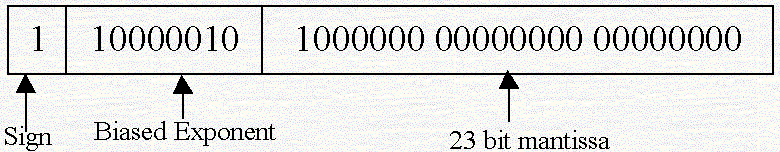
\includegraphics[width = 100mm]{img/rep.png}
        \end{figure}
        \vspace{-6pt}
        Here, the decimal number -12 is represented (precisely).
    \end{frame}
    
    \begin{frame}{Floating point precision II}   
        \beI 
            \item Handling floating point numbers in decimal notation may results in imprecise output.
            \pause
            \item[$\rightarrow$] Do not rely on standard in/out methods.
            \pause
            \item[$\rightarrow$] Treat these numbers as bit (hex) strings instead 
                \newline $\rightarrow$ full information preserved.
        \enI
        \pause
        In our case, we would represent -12 as \newline 1100 0001 0100 0000 0000 0000 0000 0000 \newline or as 0xC1400000
    \end{frame}
    
    \begin{frame}{Precision comparing}
        Finding the most significant different bit: \newline
        100111001000\alt<1>{1}{\alert{1}}001110 \uncover<2->{$\downarrow$}\newline
        100111000111\alt<1>{1}{\alert{1}}010010 \uncover<2->{$-$}\newline
        \uncover<2->{000000000000\alert{1}111100}
        \beI
           \item<3-> Measuring precision in terms of different bits.
           \item<3-> Applying this to the whole type instead of mantissa only is logically valid.
        \enI
    \end{frame}

    \begin{frame}{Sample plots}
    \begin{figure}
        \begin{minipage}[l]{50mm}
           \center
           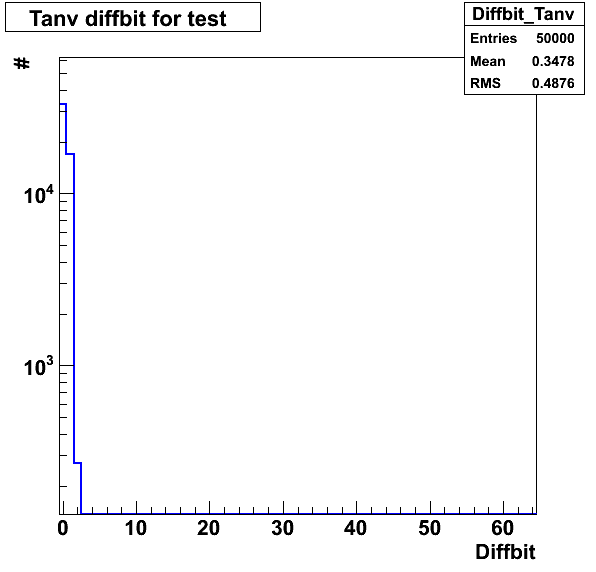
\includegraphics[width=50mm]{img/diffbit.png}
           \caption{Acceptable different bit distribution}
        \end{minipage}
        \begin{minipage}[r]{50mm}
            \center
            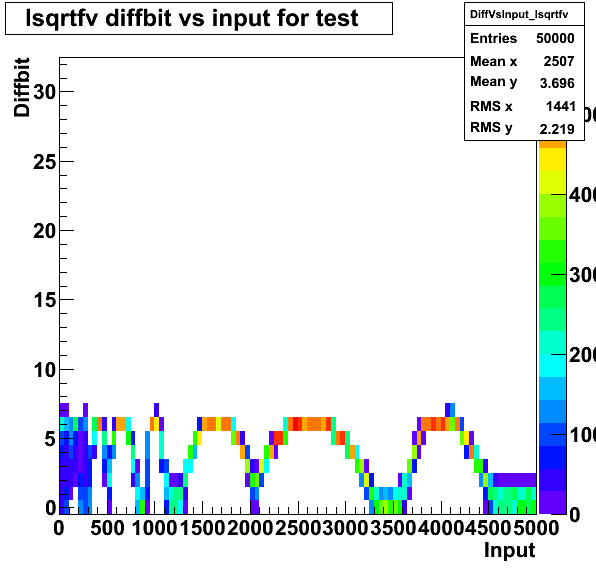
\includegraphics[width=50mm]{img/inputVSdiffbit.png}
            \caption{Fast inverse sqrt behavior (Quake III)}
        \end{minipage}
    \end{figure}
    \end{frame}
    
\subsection{Performance}
    \begin{frame}{Performance measurement}
        \beI
            \item Harder than it looks.
            \item Single function execution $\rightarrow$ nanoseconds $\rightarrow$
                impossible \newline $\rightarrow$ measure the loop across several (thousand) iterations.
            \item In many libraries you even cannot measure single function due to vector signatures.
            \item Measuring large number of iterations ($>50000$) in several trials to remove statistical fluctuations proved sufficient.
        \enI
    \end{frame}
    
\subsection{Benefits}
    \begin{frame}{Framework benefits}
        \beI
            \item Easily controllable and extendable code.
            \item Modular, decoupled stages - function response saving, arithmetic comparison, plots, performance testing.
            \item No hardcoded things (cmd options).
            \item Histograms serves as ultimate tool for possible function debugging - you can see, where the error can be.
        \enI
    \end{frame}
    
    \begin{frame}{\Cpp 11 features used}
        \beI
            \item template typedefs
            \item STL template metaprogramming ({\tt std::function}, {\tt std::tuple})
            \item constexpr - way to get rid of \#define constants
            \item auto - automatic type deduction
        \enI
        Which helps in general to:
        \beI
            \item move things from runtime to compiletime
            \item ease work with large amount of templates
            \item enhance program logic and structure without any overhead at runtime (!)
        \enI
    \end{frame}
    
     \begin{frame}{Generated file example}
        Contents of file generated by an arithmetic comparison stage (blah\_\_Asinfv\_\_comparison.txt):
         \begin{figure}
          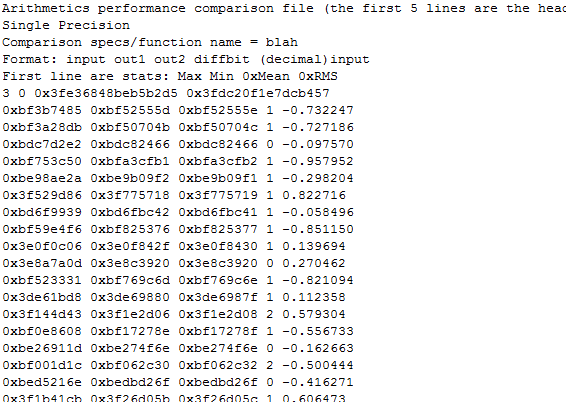
\includegraphics[width = 80mm]{img/example.png}
        \end{figure}
    \end{frame}

%\section{Custom library}
%    \begin{frame}{When writing fast math library}
%        Ways to go (simplified):
%        \beI
%            \item Trade speed for accuracy (less Taylor). Sometimes you do not need to be 100\% precise (LHC triggers).
%            \item Implement double and float separately.
%            \item Use vectorization: 
%                \beI
%                    \item Cpu can perform some SIMD operations through SSE/AVX instructions.
%                    \item Requires non-branching code.
%                    \item New compilers have autovectorization capability.
%                    \item Or... use GPU - same principle, longer story.
%                \enI
%        \enI
%    \end{frame}
    
\subsection*{}
    \begin{frame}{}
        \begin{center}
          Thank You. 
 
          Questions.
        \end{center}
        
    \end{frame}

\end{document}                                              